\documentclass[tikz,border=10pt]{standalone}
\begin{document}
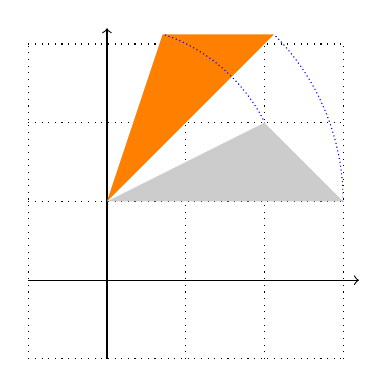
\begin{tikzpicture}
  \draw[thin,dotted] (-1,-1) grid (3,3);
  \draw[->] (-1,0) -- (3.2,0);
  \draw[->] (0,-1) -- (0,3.2);
  % original triangle:
  \fill[gray!40] (0,1) -- (3,1) -- (2,2) --cycle;
  % rotated triangle:
  \fill[orange,rotate around={45:(0,1)}]
    (0,1) -- (3,1) -- (2,2) --cycle;
  % clipped circles to show the rotation:
  \begin{scope}
    \clip (2.1,3.1) rectangle (3,1);
    \draw[blue, densely dotted] (0,1) circle(3);
  \end{scope}
  \begin{scope}
    \clip (0.72,3.2) rectangle (2,2);
    \draw[blue, densely dotted] (0,1) circle(2.24);
  \end{scope}
\end{tikzpicture}
\end{document}
